% Hauptdatei der Vorlage fuer Seminararbeiten am Lehrstuhl f{\"u}r Hochleistungsrechnen (nicht ver{\"a}ndern!)
% Veraenderungen bitte ausschliesslich in den (an den mit "HIER": 
% gekennzeichnenten Stellen) eingebundenen Dateien vornehmen

\documentclass[10pt,          % Schriftgroesse einstellen
               a4paper,       % Seitenformat w{\"a}hlen
               twocolumn,     % zweispaltiges Layout
               DIV14,         % Groesse des Satzspiegels (Warnung dazu bitte ignorieren!)
               BCOR=8mm,      % Bindekorrektur (abgestimmt auf LfBS-Bindeger{\"a}t)
               twoside        % Beidseitiger Druck
               %abstract=true, % Titel des Abstract ausgeben
              ]{scrartcl}
\usepackage{hpcseminar}
\usepackage[english]{babel}   % HIER: Im Falle des Falles "english"
\usepackage[utf8]{inputenc}  % UTF-8 (viele aktuelle Editoren unter Linux, Mac und Windows)

\usepackage[T1]{fontenc}      % u.a. Richtige Worttrennung
\usepackage{lmodern}          % Verbesserte "Computer Modern"-Schriften laden
\usepackage{graphicx}         % Grafiken einbinden
\usepackage{units}            % Einheiten setzen mit z.B. \unit[10]{MB} und \unitfrac[100]{Mbit}{s}
%\usepackage{siunitx}         % Wesentlich umfangreicheres Einheiten Paket als Ersatz f{\"u}r "units"

% In dieser Datei koennen eigene Erweiterungen eingebracht werden
% HIER: Nur wenn n{\"o}tig Datei my_includes.tex aendern
% Platz f\"{u}r eigene Erweiterungen und Definitionen

%\usepackage{XYZ}
%\newcommand{\hi}{Hallo}


%% Beginn des eigentlichen Dokumentes
%%-----------------------------------
\begin{document}

%% Ein paar wichtige Details konfigurieren
%% Ein paar wichtige Details konfigurieren
%%----------------------------------------
\title{Optimizing of CUDA Memory Management}
\author{André Merboldt}
\betreuer{Dipl.-Inf. Vorname Nachname}
\semester{Wintersemester 2015/2016}
\keywords{CUDA, optimization, synchronization, memory, unified memory}


% Titel automatisch erzeugen
\maketitle

% Abstract
\begin{abstract}
Following the increasing demand for faster compputation, we will discuss various techniques of the CUDA Runtime and optimizations of memory transfer and access patterns.\\
While CPUs are able to maintain levels of performance, GPUs can achieve higher parallelism due to the parallel concept of graphics processing. Unlike CPUs, graphics units operate at a lower frequency, but have many more cores to make up for it.\\
In order to fully make use of the massive parallelism, we have to apply several techniques like coalescing access to global memory to achieve the highest possible throughput.\\

% Automatische formatierte Ausgabe der oben angegebenen Keywords
\keywordsline
\end{abstract}

% Hier werden die Kapitel eingebunden
% HIER: weitere Kapitel in my_chapters.tex eintragen
% Hier werden die Kapitel eingebunden
% Bei Bedarf weitere Kapitel eintragen
\section{Introduction}
\label{sec:intro}
Performance optimizations of high performance GPU applications can be roughly seperated into three sections.\\
First, increasing instruction usage to maximize instruction troughput.\\
Secondly, utilize the GPU hardware to its full extent by maximizing parallelized execution.\\
Third, optimizing the memory transfer and access to achieve the highest possible memory throughput, which we will focus on later in section \ref{sec:transfer} and \ref{sec:access}.
\\
To utilize the full potential of highly parallized GPUs, also called \emph{devices},
several frameworks emerged. One of them is CUDA, developed by NVIDIA and therefore targeting only NVIDIA GPUs which
provides us with a coherent and consistent view.\\
As there are many NVIDIA GPUs on the market with different features and specifications, they have been
classified into so-called \textbf{compute capabilities} (CC). At the moment four major versions are available,
Tesla hardware with compute capability 1.x, Fermi with CC 2.x, Kepler with CC 3.x and the latest Maxwell hardware with CC 5.x.\\
CUDA itself also matured over time, so some features may only be available on later versions, where we will focus on CUDA 7.5. 
%\cite{http://docs.nvidia.com/cuda/cuda-c-programming-guide/index.html#compute-capability}
Therefore is Tesla-class hardware which is not longer supported by CUDA 7\cite{c_prog_guide_cc}, not be covered in this thesis.\\\\

% todo: other words
In the first two chapters we will lay the foundation for further thoughts with the hardware architecture  and the CUDA memory management.\\
After that, the main topic of this paper will be highlighted: the optimization of memory transfer and access.\\
%CUDA platform-independent and device-independent is an API by NVIDIA to utilize GPUs for accelerated computation.\\
%As both GPUs and CUDA itself matured over time, we will discuss CUDA at version 7.5 and highlight devices of compute capability 2.x to 5.x.\\
%To enable high performance computation, we have to efficiently pass data around and optimize access to memory.\\
%Prior to the discussion of optimization techniques, we will outline the basics of computation using GPUs with CUDA.

\section{Hardware Architecture}
\label{sec:hardware}
\subsection{Overview}
Each GPU contains several multiprocessors (current hardware up to 
In contrast to the more sequential CPU computational flow, GPUs work highly parallelized.

This parallelization is because of many more computational cores 

Due to GPU hardware having more cores than CPUs, computation is organized into threads which are meant to be executed in parallel, grouped into multiple \textbf{blocks}, called a \textbf{grid}. Both grids and threadblocks can have a dimension up to 3. Using these constructs, it is easily possible to index a multidimensional structure.\\
Grids are created upon a call of a \textbf{kernel} - that is a code sequence running on CUDA-capable devices - (?). Below is an illustrated overview of one two dimensional grid (3x3) of blocks each running a number of threads.\\
\begin{figure}
    \centering
    \includegraphics[scale=0.5]{media/threads_blocks_grid.png}
\end{figure}
\\
CUDA assigns blocks to streaming multiprocessors, 
\subsection{Memory}
\subsubsection{Device}
\paragraph{Global Memory}
\label{hardware_global}
The most ample of all GPU memory, often exceeding several gigabytes on current hardware, is accessible to all threads on the GPU and per PCIe even to the host.\\
Global memory is located off-chip, resulting in a higher latency around 500 clock cycles which is often hidden through thread parallelism but still a way higher bandwidth than the connection per PCI Express between host and device.\\
Memory transactions are used to global memory and these have to be aligned to their transaction size of 32, 64 or 128 bytes.\\
The high latency can impose a significant performance loss, to minimize its impact CUDA will try to merge as many transactions as possible. We will explore these coalescing mechanisms later in ~\ref{global_access}.\\
\paragraph{Shared Memory}
Due to being located on-chip, therefore resulting in low-latency, high-bandwidth memory, shared memory is used to exchange data between threads in a block and synchronize them.\\
Additionally shared memory is ideally suited to manually cache global memory.\\
\paragraph{Registers}
Data used without keywords (shared, global aka device) in a kernel are stored in registers, as long as they can hold it.\\
Though there are multiple thousands register (between 32K and 128K for current hardware) available for use by the compiler,
these registers have to be split between concurrently running threads on a multiprocessor.\\
Should the compiler decide that local data is too big to be hold in register only,
it will be stored in local memory which is by orders slower than registers or shared memory.\\
This phenomenon is called \emph{register pressure} and should be avoided by investigating local memory usage
and using shared memory.\\
\paragraph{Local Memory}
Contrary to its name is local memory not located on-chip, but in global memory.
Therefore it inherits its characteristics, most important the high latency which may limit an applications performance immensly.
To avoid local memory usage, the compiler supports a switch called \emph{--ptxas-options=-v} with which several information regarding
the generated code is shown. 
\paragraph{L1 Cache}
L1 Cache is on-chip memory, caching access to local memory. Shared memory and L1 cache are sharing the same memory space. \\
\paragraph{L2 Cache}
In contrast to L1 cache, L2 Cache is shared between all multiprocessors and is used to cache access to local and global memory.\\
% TODO: show when introduced etc.
\paragraph{Texture Memory \& Cache}
Texture memory can be used to hold data aswell and is optimized to store two dimensional data.\\
\subsubsection{Transfer}
GPUs are connected to a hostsystem via PCI Express, which limits the bandwidth of the memory transfer between host and device.\\
PCI Express is a point-to-point system (source?) and as data exchange is done using packets,
there is a significant overhead involved.\\
\begin{table*}
\centering
\begin{tabular}{c|c|c|c}
\textbf{Generation} &   \textbf{Transfer-Rate}      & \textbf{per Lane} & \textbf{16-lane}\\
\hline\hline
PCIe 1.0     &   2.5 GT/s               & 2 GBit/s          & 32 Gbit/s\\
PCIe 2.0     &   5.0 GT/s               & 4 GBit/s          & 64 GBit/s\\
PCIe 3.0     &   8.0 GT/s               & 7.87 GBit/s       & 126 Gbit/s\\
PCIe 4.0     &   16.0 GT/s              & 15.754 GBit/s     & 252 GBit/s\\
\hline
\end{tabular}
\caption{Comparison of different iterations of the PCI Express protocol, source: pcisig.com}
\label{tab:pci_comp}
\end{table*}
\emph{**show GPU Global memory transfer rates**}
As a comparision, GDDR5 (double rate type 5 synchronous graphics random access memory) is able to maintain a bandwith in excess over 100/200 GB/s.
\\
As we can see, the GPU memory is several times faster than the PCIe protocol theoretical maximum bandwidth.\\
This means we will have to try to minimize data transfer between host and device as PCIe is many times slower than device memory.
We will exploit this knowledge to achieve (?) high computational throughput (?).
\subsection{Kernel}
A \emph{Kernel} is a code procedure launched from the host and executed in a grid of threadblocks on the graphics unit.\\
Once the CUDA code is loaded onto the GPU, a global scheduler distributes the threadblocks to the streaming processors, in which then warp schedulers select 32 threads ( one warp ) for execution.\\

\section{Memory Management}
\label{sec:management}
\subsection{Memory Allocation}
\label{sec:mem_alloc}
We need to differentiate the allocation of host and device memory.
While we can allocate host memory using malloc, but not exclusively, device memory is generally allocated using cudaMalloc.
\emph{cudaMalloc()} can allocate a linear memory in the device memory, given the device has enough free memory.
Important to note is that \emph{cudaMalloc()} is always blocking, as an alternative can cudaMallocAsync be used which uses streams (...?).



Allocation and Deallocation are expensive operations and as a consequence we should reuse memory whereever it is possible.
(maybe show timings?)
\subsubsection{Dynamic Allocation}
Since compute capability 2.x, CUDA developers can allocate global memory in their kernels using \emph{malloc()} and operate using \emph{memset()} and \emph{memcpy()}.
\subsubsection{Pitched Layout}
Due to coalescing constrains, which we will discuss in depth in ~\ref{sec:access}, it is possible to allocate \emph{pitched memory}.\\
This memory is used for 2D and 3D memory, where the column or row number is not easily divided by a power of 2.\\
Therefore we can allocate this memory using a padding, where we use more memory than we need, but align the data in a way in which it is easily accessible.\\
Illustration:
\subsection{Streams and Synchronization}
\subsubsection{Synchronization}
In a highly parallized enviroment like CUDA, it is critical to synchronize the threads to allow benefitial collaboration.\\
CUDA provides several mechanics for developers to enable and simplify this process. CUDA applications has to synchronize on several depths, first on the threadblock level, where threads have to synchronize using shared memory and \_\_syncthreads() its work.\\
Secondly interblock synchronization can be implemented using cudaEventSynchronize() and \emph{cudaStreamSynchronize()}. Lastly (?), CUDA events may be used with \emph{cudaStreamWaitEvent()} to enable inter-GPU synchronization.\\
Additionally, there is the possibility to use atomic operations which are guaranteed to be "unteilbar"?? on device memory and are implemented by the graphics memory controller. 
\subsubsection{Streams}
\label{sec:streams}
Operations like memory copy or kernel launches are enqueued into a sequence, which is called a \emph{stream} in CUDA.\\
It is possible and often advantagous due to parallelized matters to use multiple streams which are able to run concurrently.\\
Using streams it is possible to implement for example overlapped data transfer.
\subsection{Unified Virtual Addressing}
\label{sec:uva}
Before the introduction of \emph{Unified Virtual Addressing} (UVA) in CUDA 4, address spaces of device and host were separate, which implied that every memory transfer has to specify which address space to target. (? expression)\\
UVA combines both address spaces to create a single unified virtual address space in which data from both device and host reside. This concept results in a simplified view of memory and enables the developer to stop using \texttt{cudaMemcpyDeviceToHost} and \texttt{|cudaMemcpyHostToDevice|} and use \texttt{cudaMemcpyDefault} in \emph{cudaMemcpy} methods.
Because of the unified address space, UVA only works on 64 bit operating systems, as 32 bit systems can only allocate roughly 4 GB and modern computers often exceed these limitations, especially combined with device memory.\\
UVA also enables \emph{Zero-Copy}~\ref{sec:zerocopy}.
\subsection{Unified Memory}
\label{sec:unified_memory}
\emph{Unified Memory}, introduced in CUDA 6, simplifies memory management with managed memory which is available to device and host equally.\\
With Unified Memory it is possible to allocate memory using \emph{cudaMallocManaged} and pass the pointer to a kernel, which is able to operate directly on it without the use of copies.

\section{Memory Transfer Optimization}
\label{sec:transfer}
\subsection{Pinned Memory}
\label{pinned}
One of the most important aspects of optimization is the memory transfer between host and device.\\
Unfortunely, as we have seen in \ref{tab:pci_comp}, the link bandwidth between host and device is by several times slower than access to device memory.\\
Memory transfer without modifications uses pageable memory to copy data from host to device and vice versa.\\
Using pageable memory is problematic, because as soon as the device requests access to host memory ( for example for memory copies)
the host has to check whether the data even resides in physical memory or if it has been swapped out.\\
This results in a non-trivial CPU load and therefore lowers the bandwidth.\\
To avoid this, it is possible to request so-called page-locked, or \emph{pinned memory} which is not eligible to swapping (? even access?).\\
Page-locked memory results generally in a much higher bandwidth, though this difference is influenced by the CPU where a system
with a stronger CPU performs better than a system with a weaker processor on pageable memory but in all instances slower than pinned memory.\\
Without the involvement of the processor, the OS has to fulfil the demand that page-locked memory is \textbf{always} backed by physical memory,
so the device can setup a direct memory access ( DMA).\\\\
Resulting into higher bandwidth and lower system load for the host, it is one of the simpliest yet most effective ways to improve memory transfer.\\
Using consumer-grade hardware the following data has been gathered to further display the differences in \ref{fig:bandwidth}.\\
\begin{figure*}[ht]
    \centering
    \includegraphics[scale=0.5]{media/bandwidth_pageable_vs_pinned_both.png}
    \caption{averaged bandwidth of 10 measurements on GTX 750 1GB, Intel(R) i5-4670 @ 3.40GHz}
    \caption*{Source code: \href{https://github.com/spotlight0xff/cuda\_paper/code/bandwidth}{On Github}}
    \label{fig:bandwidth}
\end{figure*}
% discuss results
These results have been recorded by allocating 128 different memory sizes (linearly distributed from 1 byte to roughly 700 MB) using respectively pageable and pinned memory.\\
To verify the data, these recordings have been averaged about 10 measurements.\\
The above figure shows clearly the significant speed-up provided by pinned memory, especially in the case of device to host transfer
whereas pinned memory shows no notable difference between the transfer direction.\\
Even though the overall results may be expected, the displayed disparity between the pageable memory transfers can be surprising. (explanation...?)\\\\

While host memory is page-locked, it can't be access and therefore used by the operating systems memory management,
which may result in degration of the systems performance due to insufficient memory available.\\
Another notable pitfall of pinned memory is the increased allocation time as we can see in the next paragraph.\\
\subsubsection{Registering Host Memory}
In some cases it is desirable to not allocate pinned memory, but to flag already allocated host memory as pinned memory.\\
This is especially interesting for applications with addon functionality where addons can provide host memory,
the application then registers it as page-locked using \emph{cudaHostRegister()}, operates on the accelerated memory and later unregister it with \emph{cudaHostUnregister()}.\\
\begin{table}
\centering
\begin{tabular}{c|c|c}
    \textbf{Size} & \textbf{Allocation} & \textbf{Registration}\\
\hline
\textbf{512 bytes} & 0.30 ms  & 0.08 ms\\
\textbf{1 MB}      & 0.28 ms  & 0.23 ms\\
\textbf{200 MB}    & 37.92 ms & 17.83 ms\\
\textbf{500 MB}    & 94.30 ms & 44.11 ms\\
\hline
\end{tabular}
\caption{Allocation times of pinned memory versus registering host memory}
\caption{System: GTX 750 1GB CC 5.0 with CUDA 7.5}
\caption{Source code: \href{https://github.com/spotlight0xff/cuda\_paper/code/alloc/}{on GitHub}}
\label{tab:host_reg_pinned}
\end{table}
As expected is marking host memory as pinned faster than allocation itself.\\
\subsubsection{Portable Pinned Memory}
Pinned Memory can be allocated or registered \emph{portable}  when it is required to access data on multiple CUDA units,
because an allocation made by one GPU is by default only accessible to the allocator.\\
As with the following two types of pinned memory, using it is as simple as setting a parameter in
\emph{cudaHostAlloc} or \emph{cudaHostRegister} to \emph{cudaHostAllocPortable} or \emph{cudaHostRegisterPortable} respectively.
Memory marked as portable is mapped and accessible by all GPUs on the system.\\
With UVA in effect, pinned memory is per default marked portable.
\subsubsection{Mapped Pinned Memory}
To map pinned memory directly into the GPU address space, enabling the developer to access 
in CUDA 2.2, it is possible to map pinned memory directly into the CUDA address space, which enables the developer to write directly to host memory.\\
This eliminates the need for device memory allocation, especially in a situation where data has to be only read or written once, it is preferable to use mapped memory instead of memory copies.\\
Using mapped pinned memory it is important to align the data properly to have its access coalesced as described in ~\ref{global_access}.
With UVA in effect, CPU and GPU share the same address space and therefore the same address can be used so there is no need to update both allocation tables.
\subsubsection{Write-Combined Pinned Memory}
TODO
\subsection{Zero-Copy}
\label{zerocopy}
Mapped Pinned Memory, or \emph{zero-copy},  is a feature introduced in CUDA 2.2 to allow direct access to host memory without explicit memory copies.\\
This is particulary useful if data is accessed sparsely or if the GPU is integrated.\\
On integrated GPUs zero-copy is always benefitial, because the host memory (most notable the RAM) and the GPU share the same physical memory. Therefore it is unnecessary to perform additional memory copies.\\
Another interesting use of mapped pinned memory is the ease with which it is possible to enable overlapping memory transfer with kernel execution.\\
Overlapping is normally performed using multiple streams where only parts of the memory is copied at once like illustrated in \ref{fig:overlapping}.\\
CUDA simplifies this process with zero-copy, where the data transfer is done transparently similar to the Unified Memory concept ( see \ref{unified_memory} ) where data is only transferred as needed.
This technique is only possible and benefitial due to DMA, because without it a host thread would've had to receive and perform the memory transfers accordingly, resulting in higher system load and lower bandwidth.\\
Additionally to overlapping, zero-copy can also be used to access complex structures without performing expensive deep copies, again similar to Unified Memory.\\

\section{Memory Access Optimization}
\label{sec:access}
% after trafer of memory
After memory transfer, it is important to access the transfered data efficiently.\\
Both access to global and shared memory obey access constraints and to fully optimize CUDA applications it is important
to follow several requirements which we will examine below.
\subsection{Global Memory Access}
%\cite{pfa_access_global}
\label{global_access}
% only mem av from host
Global memory is arguably the most important memory in a GPU with the vast amount of memory available and its global scope.\\
Though the bandwidth is very high with well over 100 GB/s on current hardware, it may be decreased heavily by uncoalesced access patterns which we will dissect now.\\
\subsubsection{Theoretical Bandwidth}
%\cite{http://devblogs.nvidia.com/parallelforall/how-implement-performance-metrics-cuda-cc/}
In evaluating and optimizating global memory access and its throughput it is useful to have a metric to compare against.\\
This can be provided by the theoretical bandwidth peak which allows approximation of device memory bandwidth capabilities. It has to be emphasized that this is only the theoretical possible bandwidth, which shows if more optimization is needed as the first optimizations can generally be quite simple.\\
$$ BW_{\mathrm{theoretical}} = CLK \times \mathrm{Width}_{\mathrm{Bus}} \times DDR $$
Where $CLK$ is the clock rate (which can vary depending on GPU boost) and $\mathrm{Width}_{\mathrm{Bus}}$ is the memory bus width and $DDR$ can be two due to double data rate used by modern GPU.\\
% todo citation
Using this formula, the theoretical bandwidth for a system with a GDDR5 memory clocked at 1.8 GHz and a 384-bit wide bus results in \SI[per-mode=symbol]{168}{\gibi\byte\per\second}.
% todo citation
%\cite{cuda_handbook_5.2.13_ecc}
The achieved bandwidth can also be lowered by error correcting code (ECC), which can correct 1-bit and report 2-bit memory errors by about $20\%$. 
\subsubsection{Coalesced Access}
As mentioned in \ref{hardware_global}, CUDA tries to merge memory requests from a warp together in order to improve global memory performance.\\
While CUDA GPUs with better hardware capabilities have emerged, the hardware and algorithms to merge memory requests have also improved,
however CUDA applications striving for high performance will still have to optimize its memory access.\\
There are several factors to pay attention to when addressing accessing global memory:\\
\begin{itemize}
    \item Only access to 1, 2, 4, 8 and 16 bytes of global memory will compile to a single instruction.
    \item Accessed data has to be naturally aligned, i.e. its address has to be a multiple of its size.
    \item Access patterns following the hardware guidelines have to be used.
    \item more-dimensional data have to aligned correctly to provide coalesced access, see \ref{2d_access} for details.
\end{itemize}

%\subsubsection{memory requests / memory transactions}
%\subsubsection{size and alignment}
% misalignment doesnt matter in cc 2.x up
\subsubsection{Aligning Structures}
Like all other global memory access, structures have to be aligned to have its access coalesced.\\
It is possible to enforce this behaviour using the compiler keyword  $\_\_align(n)\_\_$
where now the structure have its starting address aligned to a multiple of $n$.\\
Additionally, if the size of the structure is not a multiple of $n$, an array of the structure will be padded to have its size aligned as well.\\
For example the structure $testStruct$ (name...) is now aligned to at least 32 bytes:\\
\begin{lstlisting}[language=c]
struct __align__(8) testStruct {
    uint16_t a, b, c;
}
\end{lstlisting}

% todo: test!!!
% 
Normally, without the $\_\_align\_\_$ keyword, this structure would have a size of 6 bytes but to have its
size aligned to a multiple of 8, it is padded using another 2-byte word.\\

\subsubsection{Strided Memory Access}
While misaligned accesses on more current hardware have lower impact on performance than before\cite{pfa_access_global}, due to more advanced coalescing techniques and hardware,
strided access is still a problem and will continue to be challenging.\\
This comes at no surprise, because when threads in warp access memory at locations far apart, there is no way for the hardware to merge its memory requests and provide coalesced access.\\
\begin{figure}[H]
    \centering
    \includegraphics[scale=0.18,natwidth=1200,natheight=800]{media/strided_bandwidth.png}
    \caption{Strided Access on current hardware\\\hspace{\textwidth}hi test test2}
    \caption*{Test system: NVIDIA GTX 750 1GB CC 5.0, CUDA 7.5}
    \caption*{Source code: \href{https://github.com/spotlight0xff/cuda\_paper/code/coalescing\-global/}{On GitHub}\cite{pfa}}
    \label{fig:strided_access}
\end{figure}
Figure~\ref{fig:strided_access} illustrates the memory throughput using the following strided memory access pattern on 32-bit and 64-bit word sizes.\\
$$ (blockDim.x \times blockIdx.x + threadIdx.x) \times \mathrm{stride} $$
%Surprisingly, 
As expected, strided access proves to be impactful on the performance although surprisingly,
64-bit data has a higher throughput compared to 32-bit.\\
% TODO explanation or fuck off
This can be mitigated by using shared memory to manually cache the strided data in shared memory in a coalesced fashion. As we will see later, shared memory does not punish for strided access.\\
\subsubsection{Latency Hiding through Thread Parallelism}
Even though some kernels may be latency-bound,
that is when the kernel execution depends on the latency of global memory to continue execution,
this may not effect the performance using high enough block size.\\
%todo clarify
Because of how the SM schedules warps for execution,
if enough warps are waiting to be executed, some warps waiting to complete a memory request can be skipped.\\
This is only because of how lightweight threads are implemented on GPU in comparison to traditional threads on a CPU where each time a context switch is performed, registers have to be restored.
Contrary to that, on a GPU a context switch does \emph{not} perform any expensive operation as the registers are all stored on the multiprocessor and can be used directly.\\
Quoting a NVIDIA presentation, to hide math and memory latency about``~512 threads per SM'' \cite{sc11_perf_optimization} are needed.\\
%As said, each microarchitecture has different constrains, which we will discuss below.
\subsubsection{Fermi-class hardware (CC 2.x)}
%\cite{cuda_handbook_global_memory_sm2_x}
Devices of compute capability 2.x will cache global memory accesses by default in both L1 and L2 cache,
though this behaviour can be changed to cache only in L2 with a compiler switch.\\
While requests served by both L1 and L2 cache will result in 128-byte transactions, requests only operating on L2 cache result in 32-byte transactions.\\
Therefore it is sometimes useful to use only L2 cache, as in the case of scattered or random access to avoid fetching too much data.\\

%Contrary to devices of compute capability 1.x, Ferm-class hardware will coalesce access to global memory within a whole warp
%and cache by default in L1 and L2 cache, though this can be changed to caching only in L2 with a compiler switch.\\
%Caching only in L2 may be useful to reduce overfetch for scattered or random access, as L2 cache lines are only 32-byte (cache segments??)
%while L1 cache contains 128-byte cache lines and reduce therefore overfetch.

%On Fermi-class hardware is global memory access by default cached in both L1 and L2 cache.

%Beginning with Fermi, the L1 cache with lines of 128 byte are used to cache access to global memory.\\

%Global memory will be served using both caches ( though this can be changed using compiler directives, using \emph{-Xptcas -dlcm=cg} to just L2 cache), 
\subsubsection{Kepler-class hardware ( SM 3.x)}

With Kepler all global memory access is cached through L1 while L2 is reserved for local memory requests.\\
Starting with SM 3.5, chips have the capability to use the texture cache to fulfil memory requests as well.\\
\subsubsection{Maxwell-class hardware (SM 5.x)}

\subsubsection{Two Dimensional Access}
%\cite{shane_global_memory}
%\cite{http://docs.nvidia.com/cuda/cuda-c-programming-guide/index.html#device-memory-accesses}
\label{2d_access}
To use coalescing access to two-dimensional data
\footnote{I will focus on two-dimensional arrays only, but the same theory applies to data in more dimensions},
it is needed to have a correctly aligned array.
For instance if an array of 50 rows with each 30 float values is needed,
a call to cudaMalloc with the requested size of $ 50 \times 20 \times sizeof(float) $ results in a allocated memory of 4000 bytes.
The problem occurs when accessing the first element of the second row, i.e. $ values[1][0] $.
The address of this element equals the length of a row which is 50 bytes. This is not a multiple of the warp size, which may result in uncoalesced access.\\
Therefore it is desired to have arrays with dimensions according to coalescing constrains.
For convenience CUDA provides the possibility to allocate so-called \emph{pitched memory},
that is mostly more-dimensional memory with a padding aligned to meet the hardware requirements for coalesced access.\\
To use this feature, \emph{cudaMallocPitch()} and \emph{cudaMalloc3D()} are available for two-dimensional and three-dimensional arrays, respectively.\\
Indexing a pitched 2D memory works with the following formula:\\
$$ (base + row * pitch) + column$$\\
This technique allows on all hardware fully coalesced access and also transfer using \emph{cudaMemcpy2D()} and \emph{cudaMemcpy3D()}.\\
\subsection{Shared Memory Access}
\label{shared_access}
Due to being on-chip, shared memory has extremly fast access times and very high bandwidth for threads on the multiprocessor. Therefore it is mostly used to exchange and synchronize between threads in a block.\\
Shared memory is accessed using 32 memory banks, which are able to maintain a bandwidth of 32 bits every clock cycle and every two clock cycles for Fermi and Maxwell devices, respectively.\\
Kepler devices are able to switch between word sizes of 32-and 64-bit width to enable fast shared memory access to 64-bit values like $doubles$, though this mode has been dropped due to increased simplicity in Maxwell devices.\\
% todo: why dropped? + cite
This memory bank concept enables high performance concurrent access where the resulting bandwidth is 32 times higher than the bandwidth of a single memory bank given that no bank conflicts occur.\\
Memory banks are organized in a way that successive word are assigned to successive memory banks.\\
When $n$ threads with $n>1$ try to access the same bank requesting a different word, the access is serialized and the bandwidth is lowered and a $n$-way bank conflict occurs.\\
If the same word within a memory bank is accessed by all threads or multiple threads in a warp no bank conflict is generated as the value is respectively broadcasted or multicasted to the requesting threads.\\

\section{Conclusions}
\label{sec:concl}
%The discussed methods and techniques have shown how to transfer and access different kinds of memory efficiently.
%Because we can compute and access data way faster on the device than transfer it to it, it is often better/more efficient
%to do some calculations/computations on the device even if they don't get processed faster, but to avoid memory transfer.
%This results in more GPU code and therefore higher complexity. (?)
The discussed methods and techniques have shown how to transfer and access different kinds of memory efficiently.\\
We are able to compute (to a degree) and access data way faster on the device than transferring data to it.
Therefore it is often more efficient to do calculation on the device even if they do not get processed faster, but to avoid slow memory transfer.\\
NVIDIA provides useful resources and tools for profiling high performance applications like the performance analysis using the Visual Profiler\cite{visual_profiler} or \emph{nvprof}\cite{nvprof}.
This enables the developer to determine exactly where optimization can be applied.

There are of course many more optimization opportunities available which can be applied to the rapidly evolving field of GPU computing with a great number of applications like computational fluid dynamics\cite{computational_fluid_dynamics}, machine learning\cite{machine_learning} or data science\cite{data_science}.\\
All these fields benefit heavily from the accelerated computing performed by GPUs and therefore it is most likely that for even higher computational power is pushed.\\



% Das Literaturverzeichnis erzeugen
% HIER: Eintraege in literatur.bib hinzufuegen
\bibliographystyle{alpha}
\bibliography{literatur}

\end{document}
